\documentclass[tikz,border=6pt]{standalone}
\usepackage[T1]{fontenc}
\usepackage[utf8]{inputenc}
\usepackage{pgfplots}
\usepgfplotslibrary{groupplots}
\usetikzlibrary{calc}
\pgfplotsset{compat=1.18}
\begin{document}
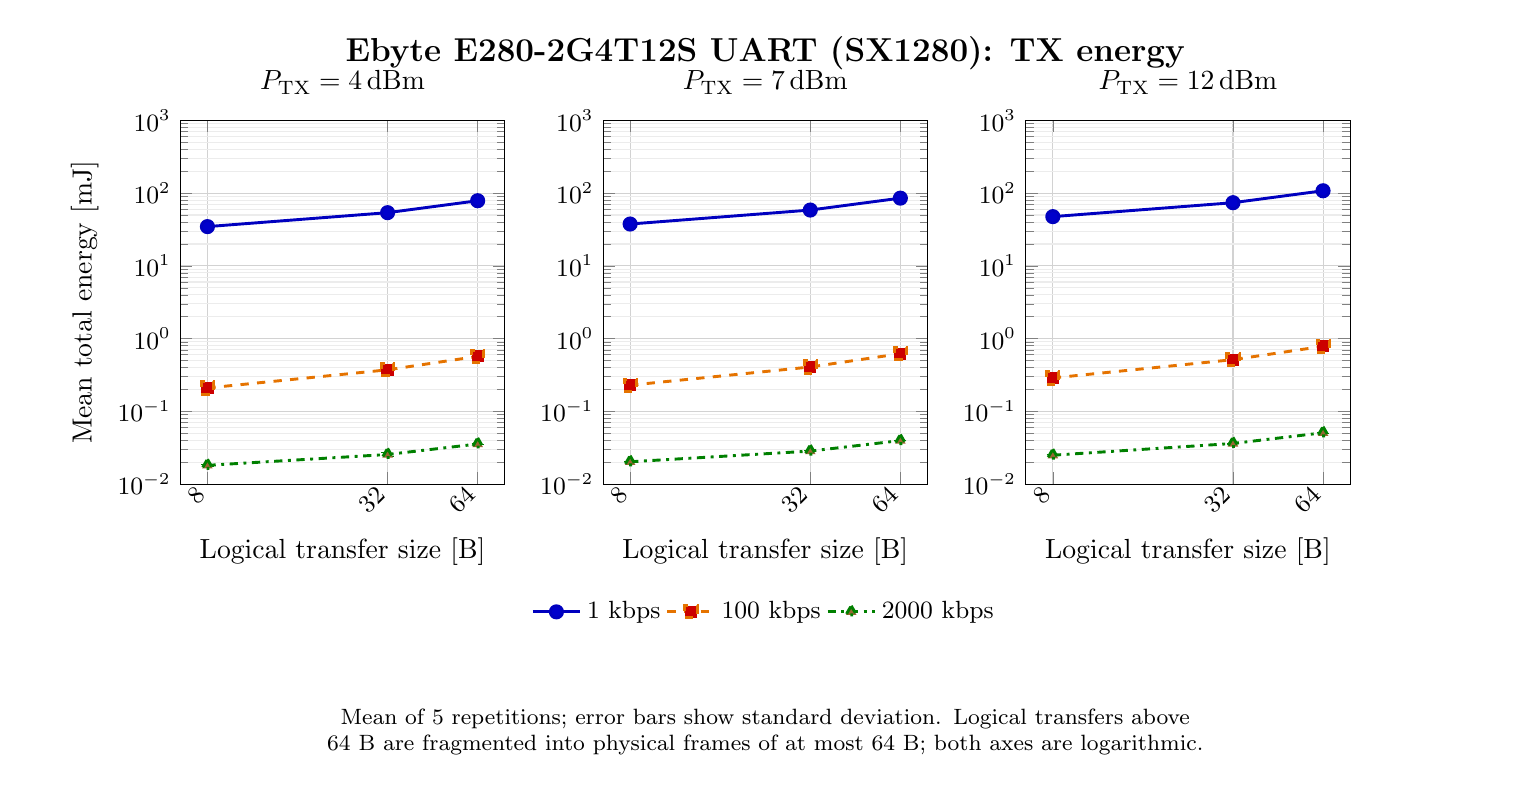
\begin{tikzpicture}
\begin{groupplot}[/pgf/number format/use comma,
  group style={group size=3 by 1, horizontal sep=1.25cm},
  width=5.7cm, height=6.2cm,
  xmode=log, log basis x={2}, ymode=log, log basis y={10},
  ymin=0.01, ymax=1000,
  xtick={8,32,64}, xticklabels={8,32,64},
  x tick label style={rotate=45, anchor=east, font=\small},
  y tick label style={font=\small},
  grid=both, minor grid style={gray!15}, major grid style={gray!35},
  xlabel={Logical transfer size [B]},
  every axis plot/.append style={line width=1.05pt},
  error bars/error bar style={line width=0.35pt},
  legend style={font=\small, draw=none, fill=none, at={(0.5,-0.29)},
    anchor=north, legend columns=-1},
]
\nextgroupplot[title={\(P_{\mathrm{TX}}=4\,\mathrm{dBm}\)}, ylabel={Mean total energy [mJ]}]
\addplot+[
  color=blue!75!black, solid, mark=*, mark size=2.2pt,
  error bars/.cd, y dir=both, y explicit,
] coordinates {
  (8,34.6715283) +- (0,0.023082692)
  (32,53.9212825) +- (0,0.0243172055)
  (64,78.6721742) +- (0,0.0756001355)
};
\addplot+[
  color=orange!90!black, dashed, mark=square*, mark size=2.2pt,
  error bars/.cd, y dir=both, y explicit,
] coordinates {
  (8,0.209494352) +- (0,0.000736765621)
  (32,0.372375999) +- (0,0.00186990055)
  (64,0.569451201) +- (0,0.000660798178)
};
\addplot+[
  color=green!50!black, dashdotted, mark=triangle*, mark size=2.2pt,
  error bars/.cd, y dir=both, y explicit,
] coordinates {
  (8,0.0181006254) +- (0,0.000518170064)
  (32,0.0255161041) +- (0,0.00137467636)
  (64,0.0355661862) +- (0,0.000514285512)
};
\nextgroupplot[title={\(P_{\mathrm{TX}}=7\,\mathrm{dBm}\)}]
\addplot+[
  color=blue!75!black, solid, mark=*, mark size=2.2pt,
  error bars/.cd, y dir=both, y explicit,
] coordinates {
  (8,37.6364617) +- (0,0.0364622551)
  (32,58.5800919) +- (0,0.026829479)
  (64,85.3871553) +- (0,0.0446117068)
};
\addlegendentry{1 kbps}
\addplot+[
  color=orange!90!black, dashed, mark=square*, mark size=2.2pt,
  error bars/.cd, y dir=both, y explicit,
] coordinates {
  (8,0.228676546) +- (0,0.000797732527)
  (32,0.40736448) +- (0,0.000877541544)
  (64,0.620105776) +- (0,0.00121154479)
};
\addlegendentry{100 kbps}
\addplot+[
  color=green!50!black, dashdotted, mark=triangle*, mark size=2.2pt,
  error bars/.cd, y dir=both, y explicit,
] coordinates {
  (8,0.0202508137) +- (0,0.000341951914)
  (32,0.0284086176) +- (0,0.000329419659)
  (64,0.0396054761) +- (0,0.00019031865)
};
\addlegendentry{2000 kbps}
\nextgroupplot[title={\(P_{\mathrm{TX}}=12\,\mathrm{dBm}\)}]
\addplot+[
  color=blue!75!black, solid, mark=*, mark size=2.2pt,
  error bars/.cd, y dir=both, y explicit,
] coordinates {
  (8,47.5503096) +- (0,0.0422337063)
  (32,73.9213755) +- (0,0.0597726522)
  (64,107.849292) +- (0,0.0578001201)
};
\addplot+[
  color=orange!90!black, dashed, mark=square*, mark size=2.2pt,
  error bars/.cd, y dir=both, y explicit,
] coordinates {
  (8,0.287714922) +- (0,0.000807942441)
  (32,0.513476392) +- (0,0.00102892613)
  (64,0.783846609) +- (0,0.00161794799)
};
\addplot+[
  color=green!50!black, dashdotted, mark=triangle*, mark size=2.2pt,
  error bars/.cd, y dir=both, y explicit,
] coordinates {
  (8,0.0249253049) +- (0,0.000234715506)
  (32,0.0361585568) +- (0,0.000424996495)
  (64,0.0507386205) +- (0,0.00049482721)
};
\end{groupplot}
\node[font=\bfseries\large] at ($(group c2r1.north)+(0,0.85cm)$)
  {Ebyte E280-2G4T12S UART (SX1280): TX energy};
\node[font=\footnotesize, align=center, text width=18.5cm]
  at ($(group c2r1.south)+(0,-3.15cm)$)
  {Mean of 5 repetitions; error bars show standard deviation. Logical transfers above 64 B are fragmented into physical frames of at most 64 B; both axes are logarithmic.};
\end{tikzpicture}
\end{document}
